\documentclass[a4paper,10pt]{article}
%\usepackage[latin1]{inputenc} % Paquetes de idioma
\usepackage[utf8]{inputenc} % Paquetes de idioma (Este encoding toma acentos :) )
\usepackage[spanish]{babel} % Paquetes de idioma
\usepackage{graphicx} % Paquete para ingresar gráficos
\usepackage{grffile}
\usepackage{hyperref}
\usepackage{fancybox}
\usepackage{amsmath}
\usepackage{amsfonts}
\usepackage{listings}
\usepackage{float}
% Paquetes de macros de Circuitos
%\usepackage{pstricks}
\usepackage{tikz}

% Encabezado y Pié de página
\usepackage{fancyhdr} % Paquete para encabezados y pie de página
\pagestyle{fancy} % Sin esta línea no se imprimiría el encabezado en todas las páginas

\fancyhf{} %  Borra el encabezado anterior (Por defecto escribe el títutlo de la sección en la que se encuentra la hoja
\setlength{\headheight}{22.55pt}
\fancyhead[L]{
	{\textsf{Facultad de Ingenier\'ia $-$ Universidad de Buenos Aires \\ 66.44 Instrumentos Electrónicos}}
}
%\addtocounter{page}{5}
\fancyhead[R]{\thepage}

\renewcommand{\footrulewidth}{0.4pt} % Ajusta el tamaño de las líneas separadoras en el pié de página
\renewcommand{\headrulewidth}{0.4pt} % Ajusta el tamaño de las líneas separadoras en el encabezado

\fancyfoot[L]{
	{\textsf{Trabajo Pr\'actico N$^{\circ}4$}: Mediciones de impedancias} \\
	{\textsf{Integrantes: Eduardo Sanchez, Francisco Soler}}
	}
		

% Carátula del Trabajo
\title{ \author{} % Lo pongo para que el warning no moleste :p
\setlength{\unitlength}{1cm} %  Especifica la unidad de trabajo
\thispagestyle{empty}

\begin{picture}(18,0)
\put(0,0){
\includegraphics[width=1.5cm, height=3cm]{Logo1.png}}

\put(10.5,0){
\includegraphics[width=3cm, height=3cm]{Logo2.png}}

\end{picture}
\\[1.5cm]
\begin{center}
	\textbf{{\Huge Facultad de Ingenier\'ia \\ Universidad de Buenos Aires}}\\[2cm]
	{66.44 Instrumentos Electrónicos}\\[0.5cm]
	{Trabajo Pr\'actico N$^{\circ}3$: Mediciones de impedancias}\\[2.5cm]
\end{center}

\begin{flushleft}
	\textbf{Integrantes:} \\[1cm]

	\begin{tabular}{|c|c|c|}
		\hline
		\textbf{\normalsize Padr\'on} & \textbf{\normalsize Nombre} & \textbf{\normalsize Email} \\
		\hline
		\normalsize 92903 & \normalsize Sanchez, Eduardo Hugo & \normalsize hugo\_044@hotmail.com \\
		\hline
		\normalsize 91227 & \normalsize Soler, Jos\'e Francisco & \normalsize francisco.\_tw@hotmail.com \\
		\hline
		\normalsize xxx & \normalsize Wawrynczak, Claudio  & \normalsize claudiozak@gmail.com \\
		\hline
	\end{tabular}
\end{flushleft}
\date{} % Hace que no se imprima la fecha en la cual se compilo el .tex
 }

\begin{document}
	\maketitle % Hace que el título anterior sea el principal del documento
	\newpage

	\tableofcontents % Esta línea genera un indice a partir de las secciones y 
					 % subsecciones creadas en el documento
	\newpage


	\section{Objetivo}
	
	\indent	El objetivo del presente trabajo práctico es familiarizarse con 
	el Q-metro, el RLC meter, el impedancímetro vectorial. Dicho instrumental
	sirve para medir impedancias. Luego de realizas las experiencias se 
	intentará determinar en qué circunstancias conviene utilizar uno en vez 
	de otro.

	\newpage
	\section{Desarrollo}
	
	\indent Para llevar a cabo las mediciones, se utilizan los siguientes 
	instrumentos:
		\begin{itemize}
			\item Q-metro 4342A Hewlett Packard
			\item LCR 819 GW Instek
			\item Impedanc\'imetro 4815A Hewlett Packard
			\item Puente de impedancias
			\item Contador
			\item Cable coaxil para realizar las distintas conexiones entre 
			instrumentos.
		\end{itemize}	
	
		\subsection{Mediciones con el Q-metro}
		\subsubsection{Inductancia de una bobina con n\'ucleo de aire}
		
		\indent El circuito simplificado de un Q-metro se muestra en la Figura
		\ref{img001}

			\begin{figure}[!htb]
				\centering
				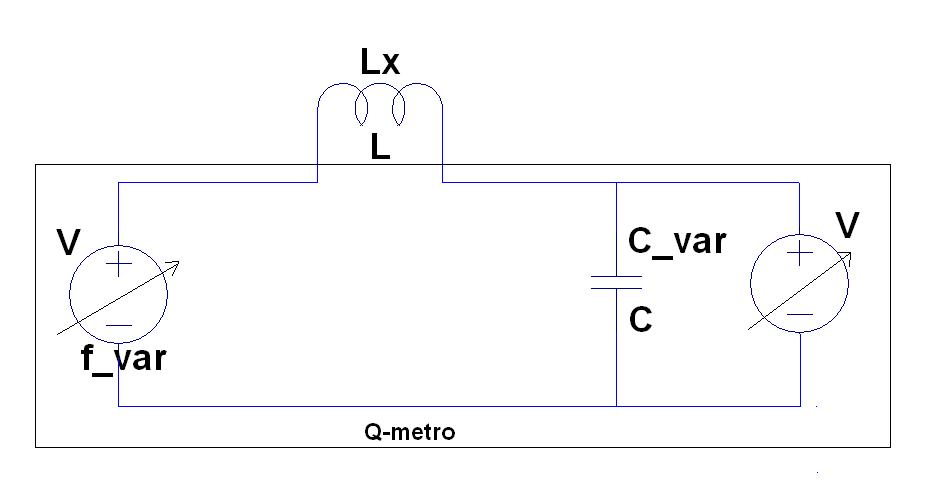
\includegraphics[width=8cm]
				{Imagenes/qmetro.png}
				\caption{Esquema simplificado del Q-metro}
				\label{img001} 
			\end{figure}

		\indent Como es un circuito serie, la máxima corriente se obtiene en 
		la resonancia, dado que la reactancia inductiva de la bobina se 
		cancela con la capacitiva. Si fuesen componentes ideales, la corriente
		sería infinita y los valores de tensiones de la bobina y del capacitor
		serían $+\infty$ y $-\infty$ respectivamente. \\
		\indent Como no son componentes ideales, los mismos tienen pérdidas y
		se las modelizan con una resistencia, por ende, la corriente no es 
		infinita. La respectiva tensión del capacitor en situación de 
		resonancia es $V_c = \frac{X_L\cdot V}{R}$. \\
		\indent Como el valor de Q es $Q=\frac{\omega L}{R}$, se observa que 
		$$V_c = Q \cdot V$$

		\indent La frecuencia de resonancia se la puede determinar de la 
		siguiente forma
		$$|X_L|=|X_C| \Rightarrow w\cdot L = \frac{1}{w\cdot C}$$

		$$f=\frac{1}{2\pi\sqrt{LC}}$$ 
		
		\indent Conocidos los valores de la capacidad, $C$, y la frecuencia, 
		$f$, puede obtenerse el valor de la inductancia de $L_x$ y tambi\'en 
		su resistencia serie equivalente con las siguientes expresiones
		$$L=\frac{1}{(2\pi)^2 f^2C}+\epsilon_L\cdot L$$
		Donde $\epsilon_L=2\epsilon_f+\epsilon_C=2\cdot 1.5\%+\frac{0.1pF}{C}$, puede calcularse a partir de las especificaciones del  fabricante.
		
		$$R_s=\frac{2\pi\cdot f\cdot L}{Q}+\epsilon_{R_s}\cdot R_s$$
		Donde $\epsilon_{R_s}=\epsilon_f+\epsilon_Q= 1.5\%+ 7\%=8.5\%$ se obtiene tambi\'en de las especificaciones del fabricante.
		\\
		\indent En la Tabla \ref{tab001} se muestran los resultados obtenidos
		para un inductor realizando un barrido de frecuencias.
		
		%Faltan incertezas jeje -----> hacete el vivo ¬¬
		%nonoo pasa que no podia abrir el manual que esta en .djvu jajaja
		\begin{table}[!htp]
					\centering
					\begin{tabular}{|c|c|c|c|c|}
						\hline
			    		Frecuencia & C & Q & L (calculado) & $R_s$ (calculado) \\
						\hline
						$13.3~MHz~\pm1.5\%$& $25~pF~\pm0.1pF$& $182~\pm7\%$ & $5.73~\mu Hy~\pm3.40\%$ &$ 2.63~\Omega~\pm8.5\%$ \\
						\hline
						$10.7~MHz~\pm1.5\%$& $40~pF~\pm0.1pF$& $200~\pm7\%$ & $5.54~\mu Hy~\pm3.25\%$ &$ 1.86~\Omega~\pm8.5\%$ \\
						\hline
						$9.6~MHz~\pm1.5\%$& $50~pF~\pm0.1pF$& $200~\pm7\%$ & $5.50~\mu Hy~\pm3.20\%$ &$ 1.66~\Omega~\pm8.5\%$ \\
						\hline  
						$6.9~MHz~\pm1.5\%$& $100~pF~\pm0.1pF$& $195~\pm7\%$ & $5.33~\mu Hy~\pm3.10\%$ &$ 1.18~\Omega~\pm8.5\%$ \\
						\hline  										
						$4.0~MHz~\pm1.5\%$& $305~pF~\pm0.1pF$& $170~\pm7\%$ & $5.20~\mu Hy~\pm3.03\%$ &$ 0.77~\Omega~\pm8.5\%$ \\
						\hline
						$3.2~MHz~\pm1.5\%$& $470~pF~\pm0.1pF$& $155~\pm7\%$ & $5.17~\mu Hy~\pm3.02\%$ &$ 0.68~\Omega~\pm8.5\%$ \\
						\hline  						  	  
					\end{tabular}
					\caption{Mediciones con el Q-metro} \label{tab001}
				\end{table}		
		De la Tabla puede observarse que las mediciones de inductancia tienen una incerteza baja (menor al $4\%$ en todos los casos) y que la mayor parte de su incerteza est\'a compuesta por la incerteza de la frecuencia. Con lo cual utilizando un instrumento que determine la frecuencia con menor incerteza (como un frecuenc\'imetro) se mejora notablemente la incertidumbre de la inductancia. Esto se realiza, obteniendose una incerteza menor al $ 1\%$ en todos los casos.
		Por otra parte, los resistencias serie equivalente calculadas tienen un grado de dispersi\'on mayor que en el caso anterior. Esto ocurre principalmente a medida que la frecuencia aumenta ya que empieza a hacerse notar el efecto capacitivo par\'asito que presenta el inductor (notar de la Tabla que el valor de Q alcanza un m\'aximo y que luego debe disminuir hasta 0 cuando alcanza la frecuencia de resonancia).
		Adem\'as se obtiene con una incerteza dominada principlmemente por la incerteza del factor Q (que es el $7\%$). Con lo cual si se desea obtener una incerteza menor deber\'a elegirse otro instrumento que no tenga un piso de incertidumbre.
		\subsection{Mediciones con el RLC}		
		%TODO, colocar que hay que calibrarlo previamnete utilizando 
		% cortocircuito y circuito abierto para determinar la impedancia serie
		% y la admitancia paralela
		Es importante antes de comenzar a medir con el RLC, realizar su calibraci\'on. De esta forma se consideran las impedancias residuales serie y paralela que se a\~naden a la impedancia a medir. Para ello deben dejarse la puntas del instrumento abiertas (para medir la admitancia residual) y en cortocircuito (para medir la impedancia serie residual).
		\subsubsection{Inductancia de una bobina con n\'ucleo de aire}
		\indent En la Tabla \ref{tabRLCbobina} se puede observar los resultados 
		obtenidos de la medici\'on de una bobina con nucleo de aire a diferentes
		frecuencias, usando el RLC. De ella puede notarse que los valores de 
		inductancia obtenidos son pr\'oximos al valor de referencia y al de las 
		mediciones realizadas con el Q-metro (ver Tabla \ref{tab001}). Sin 
		embargo, debe notarse que a diferencia de los valores obtenidos con el 
		Q-metro , el RLC tiene una incerteza un orden menor, con lo cual resulta
		ser un instrumento m\'as exacto. \\
		\indent Pero, por otra parte, posee la desventaja de tener un rango 
		limitado de frecuencias de operaci\'on (desde $12~Hz$ hasta 
		$100.00~kHz$) con lo cual resulta imposible caracterizar su 
		comportamiento en altas frecuencias. \\
		\indent Respecto al valor de la resistencia equivalente, si bien su 
		valor se calcula empleando las f\'ormulas utilizadas previamente, este 
		valor figura en una segunda pantalla del instrumento y su incerteza se 
		especifica al $0.05\%$
		%TODO huguito en la tabla tenes +- 0,5%, eso está mal, tenés que 
		% espcificarlo con el valor absoluto manteniendo las unidades
		% de donde sale la incertidumbre relativa 0.05%? en el cuadro tenés 0.5%
		%fijate en el manuaaaaaaaaaaaaaaal, una vez que esta encendido 30minutos y a temperatura entre 18 y 28 te dice que todo tiene esa incertidumbre relativa.
		\begin{table}[!htp]
			\centering
			\begin{tabular}{|c|c|c|c|}
				\hline
				Frecuencia & Q & L  & R (calculado) \\
				\hline
				$100.000~kHz$& $36.58~\pm0.5\%$ & $5.23~\mu Hy~\pm0.5\%$ &$ 89.8~m\Omega$ \\
				\hline
				$66.660~kHz$& $29.44~\pm0.5\%$ & $5.26~\mu Hy~\pm0.5\%$ &$ 74.8~m\Omega$ \\
				\hline
				$50.000~kHz$& $25.11~\pm0.5\%$ & $5.29~\mu Hy~\pm0.5\%$ &$ 66.2~m\Omega$ \\
				\hline  
				$40.000~kHz$& $22.42~\pm0.5\%$ & $5.31~\mu Hy~\pm0.5\%$ &$ 59.5~m\Omega$ \\
				\hline  										
				$28.572~kHz$& $19.07~\pm0.5\%$ & $5.35~\mu Hy~\pm0.5\%$ &$ 50.4~m\Omega$ \\
				\hline
				$20.000~kHz$& $16.10~\pm0.5\%$ & $5.40~\mu Hy~\pm0.5\%$ &$ 42.1~m\Omega$ \\
				\hline  
				$10.000~kHz$& $10.78~\pm0.5\%$ & $5.46~\mu Hy~\pm0.5\%$ &$ 31.8~m\Omega$ \\
				\hline 										
				$1.000~kHz$& $1.36~\pm0.5\%$ & $5.53~\mu Hy~\pm0.5\%$ &$ 25.5~m\Omega$ \\
				\hline 	  
			\end{tabular}
			\caption{Mediciones con el RLC} \label{tabRLCbobina}
		\end{table}
				
		\subsubsection{Capacidad de un capacitor electro\'itico}	
		\indent Para esta medición se realió un barrido en frecuencia 
		manteniendo la tensión constante y un barrido de tensión manteniendo la
		frecuecia constante. De esta forma se puede conocer cómo varía 
		
		\subsubsection{Capacidad de un capacitor cer\'amico}
		
		\subsection{Mediciones con el puente de impedancias}
		\subsubsection{Inductancia de una bobina con n\'ucleo de aire}
		En la Tabla \ref{tabPUENTEbobina}
		\begin{table}[!htp]
			\centering
			\begin{tabular}{|c|c|c|c|c|}
				\hline
				Frecuencia & Q & L  & R (calculado) \\
				\hline
				$20~kHz$& 20 & $5.10~\mu Hy$ &$ 32~m\Omega$ \\
				\hline
				$1~kHz$& 1.8 & $6.30~\mu Hy$ &$ 22~m\Omega$ \\
				\hline	  
			\end{tabular}
			\caption{Mediciones con el puente de impedancias.} \label{tabPUENTEbobina}
		\end{table}	
		
		
		\subsection{Mediciones con el impedanc\'imetro}
		Hay igual que con el RLC es necesario calibrar el impedanc\'metro antes de realizar una medici\'on usando socket Probe Check.
		Con este instrumento, para mediciones de resistencia la incerteza relativa se calcula como
		$$\epsilon_R=4\%\pm(\frac{f}{30~MHz}+\frac{R}{25~k\Omega})\%$$
		Mientras que para mediciones de \'angulo la incerteza relativa se calcula como
		$$\epsilon_\phi=3\%\pm(\frac{f}{30~MHz}+\frac{R}{25~k\Omega})\%$$
		Por otra parte las mediciones de impedancia incluyen tambi\'en efectos resuidales a la impedancia $Z_x$ que se desea medir. Este error sistem\'atico se puede observar en la Figura \ref{impres}, notando que incluye una impedancia serie $Z_s=0.5\Omega+j\cdot\omega\cdot8nHy$ y una admitancia en paralelo a $Z_x$ de $Y_p=j\cdot\omega\cdot0.3pF$
					\begin{figure}[!htb]
						\centering
						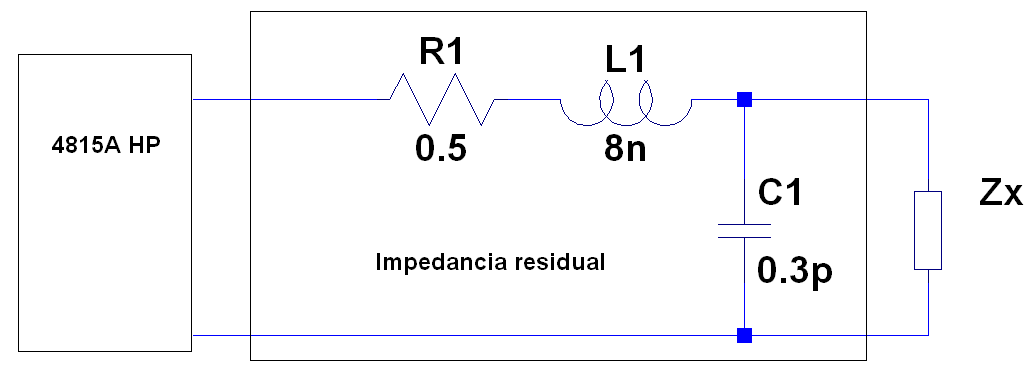
\includegraphics[width=8cm]
						{Imagenes/impedanciares.png}
						\caption{Impedancia residual del impedanc\'imetro.}
						\label{impres} 
					\end{figure}\\
		De esta forma es posible eliminar este error sistem\'atico y obtener el valor de $Z_x$, a partir del valor medido, $Z_m$, mediante la siguiente expresi\'on
		$$Z_x=\frac{Z_m-Z_s}{1-Y_p(Z_m-Z_s)}$$
		\subsubsection{Frecuencia de resonancia de una bobina con n\'ucleo de aire}
		La frecuencia de resonancia se obtiene cuando la parte reactiva de la impedancia a medir tiene fase nula, es decir, cuando
		$$\omega\cdot L=\frac{1}{\omega \cdot C}$$
		\\Con lo cual, conocida la frecuencia de resonancia y asumiendo que la inductancia no var\'ia demasiado con la frecuencia puede obtenerse la capacidad equivalente del modelo (el cual se puede observar en la Figura \ref{inductorequiv}). De esta manera
		
		$$C=\frac{1}{\omega^2 \cdot L}+\epsilon_C \cdot C$$
		Donde $\epsilon_C=2\epsilon_w+\epsilon_L\approx \epsilon_L =3.40\%$, ya que la incerteza de la frecuencia (obtenida con un frecunec\'imetro) es mucho menor a la de la inductancia (obtenida con el Q-metro en $f=13.3~MHz$)
		De esta manera se hall\'o la frecuencia ($f_resonancia=35.440~MHz$) para la cual es obtuvo fase nula y se calcul\'o la capacidad equivalente
		$$C=\frac{1}{(2\pi 35.440~MHz)^2 \cdot L}\pm \epsilon_C \cdot C=3.52pF \pm~3.40\%$$
			\begin{figure}[!htb]
				\centering
				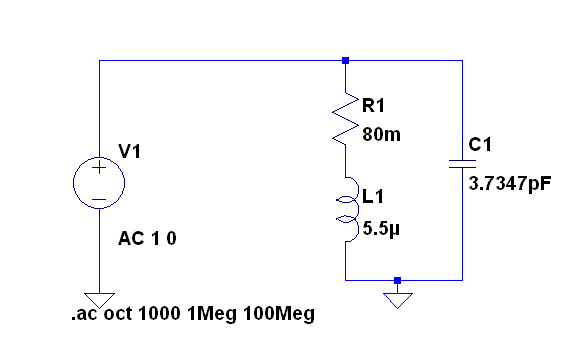
\includegraphics[width=8cm]
				{Imagenes/induceqquiv.png}
				\caption{Modelo equivalente del inductor.}
				\label{inductorequiv} 
			\end{figure}
			En la Figura \ref{respfreq} se puede observar una simulaci\'on realizada con el modelo equivalente, donde se puede observar la impedancia en funci\'on de la frecuencia y la resonancia en $f_resonancia$.
			\begin{figure}[!htb]
				\centering
				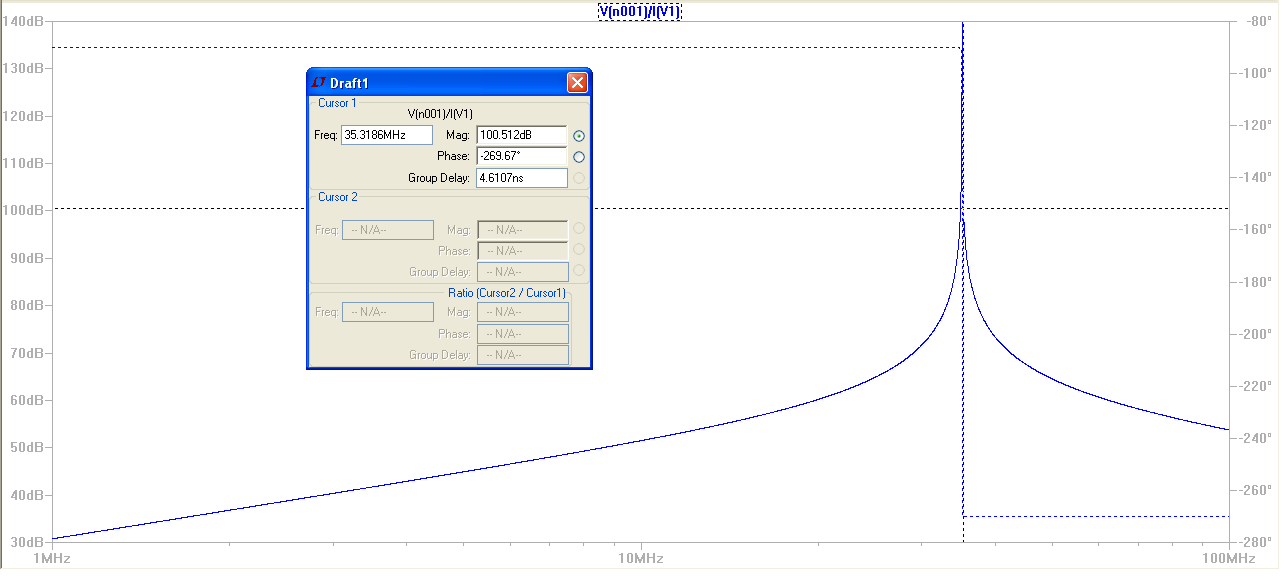
\includegraphics[width=9cm]
				{Imagenes/respfreq.png}
				\caption{Respuesta en frecuencia t\'ipica de un inductor.}
				\label{respfreq} 
			\end{figure}
		\subsubsection{Inductancia de una bobina con nucleo de ferrite}
		En la Tabla \ref{tabIMPbobina} se muestran los resultados obtenidos en m\'odulo y fase para un barrido en frecuencia entre $25~MHz$ a $100~MHz$. Debe notarse que hasta una frecuencia de  $42~MHz$, la bobina contin\'ua comport\'andose como un inductor de inductancia $L=\frac{\left|Z\right|}{2\pi\cdot f}~\pm~\epsilon_L\cdot L$. Donde $\epsilon_L=\epsilon_f+\epsilon_{\left|Z\right|}\approx\epsilon_{\left|Z\right|}$
		\begin{table}[!htp]
			\centering
			\begin{tabular}{|c|c|c|c|}
				\hline
				Frecuencia & $\left|Z\right|$ & arg(Z)  & L (calculado) \\
				\hline
				$25.5~MHz$ & $160~\Omega~\pm~4.9\%$ & $90^{\circ}~\pm~3.9\%$ & $0.99~\mu Hy$ \\
				\hline
				$42~MHz$ & $260~\Omega~\pm~5.4\%$ & $90^{\circ}~\pm~4.4\%$ & $0.98~\mu Hy$\\
				\hline
				$44.8~MHz$ & $300~\Omega~\pm~5.5\%$ & $85^{\circ}~\pm~4.5\%$ & $1.06~\mu Hy$ \\
				\hline
				$58.2~MHz$ & $430~\Omega~\pm~6.0\%$ & $78^{\circ}~\pm~5.0\%$ & $1.17~\mu Hy$ \\
				\hline									
				$69.5~MHz$ & $560~\Omega~\pm~6.3\%$ & $72^{\circ}~\pm~5.3\%$ & $1.28~\mu Hy$ \\
				\hline									
				$80.0~MHz$& $640~\Omega~\pm~6.7\%$ & $55^{\circ}~\pm~5.7\%$ & $1.27~\mu Hy$ \\
				\hline									
				$84.0~MHz$ & $550~\Omega~\pm~6.8\%$ & $45^{\circ}~\pm~5.8\%$ & $1.04~\mu Hy$ \\
				\hline									
				$93.0~MHz$ & $430~\Omega~\pm~7.1\%$ & $70^{\circ}~\pm~6.1\%$ & $0.73~\mu Hy$ \\
				\hline									
				$100.0~MHz$ & $750~\Omega~\pm~7.4\%$ & $65^{\circ}~\pm~6.4\%$ & $1.19~\mu Hy$ \\
				\hline			
			\end{tabular}
			\caption{Mediciones con el impedanc\'imetro de una bobina con n\'ucleo de ferrite} \label{tabIMPbobina}
		\end{table}	
		Si se utiliza la f\'ormula para eliminar el error siste\'atico de la medic\'on se obtiene que (para la frecuencia de 42 MHz, donde todav\'ia se comporta como un inductor)
		$$Z_x=-0.48\Omega+j\cdot 252\Omega$$
		Es decir, se obtiene una inductancia de $L=0,96 \mu F$ y una resistencia negativa, la cual probablemente se deba a la incerteza del instrumento en la fase ocacionando que el fasor de impedancia que idealmente tiene una fase de 90 grados, tenga una parte real negativa. Se puede concluir que no es un buen instrumento para medir la resistencia serie equivalente de un inductor, pero si lo es para medir inductancias.
		Por otra parte debe notarse que el barrido en frecuencia continua luego de los 42 MHz, sin embargo no se llega a alcanzar la frecuencia de resonancia donde la fase es nula. Es decir que la transici\'on de fase no es abrupta, lo cual indica que la resistencia serie es de mayor orden que la de la bobina con n\'ucleo de aire. 
		\subsubsection{Param\'etros de una l\'inea de transmisici\'on}
		Como la impedancia de entrada de una l\'inea de transmisi\'on (la que mide el impedanc\'imetro) est\'a dada por $$Z_{in}=Z_0\frac{Z_L+Z_0\tanh(\gamma L)}{Z_0+Z_L\tanh(\gamma L)}$$
		Suponiendo que la l\'inea es de bajas p\'erdidas $\gamma=\alpha+j\beta=j\beta=j\frac{2\pi}{\lambda}$ y si adem\'as se impone la condici\'on de que $L=\frac{\lambda}{8}$ entonces la expresi\'on de la impedancia de entrada se reduce a la siguiente
		$$Z_{in}=Z_0\frac{Z_L+jZ_0}{Z_0+jZ_L}$$
		Si $Z_L= 0$ entonces $Z_{in}=jZ_0$ \\
		Si $Z_L \rightarrow \infty$ entonces $Z_{in}\rightarrow-jZ_0$
		Entonces conectando una l\'inea al impedanc\'imetro a una frecuencia adecuada y dejando el extremo libre de la l\'inea cortocircuitado o abierto se obtiene el valor de la impedancia de la l\'inea, la cual es de $Z_0=75~\Omega$ ($f=7.9~MHz$ $L=3~m$)
		
		Por otra parte se si se elije $L=\frac{\lambda}{2},3\frac{\lambda}{2}, 5\frac{\lambda}{2} ...$ y que $Z_L\rightarrow\infty$, entonces puede obtenerse la atenuaci\'on de la l\'inea
		$$Z_{in}=Z_0\frac{Z_L+Z_0\alpha L}{Z_0+Z_L\alpha L}=\frac{Z_0}{\alpha L}$$
		Despejando la atenuaci\'on de la l\'inea se obtiene
		$$\alpha=\frac{Z_0}{Z_{in} L}$$
		o la atenuaci\'on en decibles cada $100~m$
		$$\alpha=\frac{Z_0\cdot8.69~dB}{100Z_{in} L}$$
		
		Con la misma l\'inea de $3~m$ con una frecuencia de $32~MHz$ se obtuvo 
		una $Z_{in}=2750~\Omega$ con lo cual $\alpha=80 mdB/m$
		
		\subsubsection{Par\'ametros de un cristal}	
		\indent Un cristal se lo puede modelar como un capacitor en paralelo a 
		múltiples circuitos RLC serie, cada uno representa un modo de resonancia
		distinto, a efectos de este trabajo práctico sólo se lo modelará con un 
		único modo de resonancia, como se muestra en la figura \ref{img004}

		\begin{figure}[!htb]
			\centering
			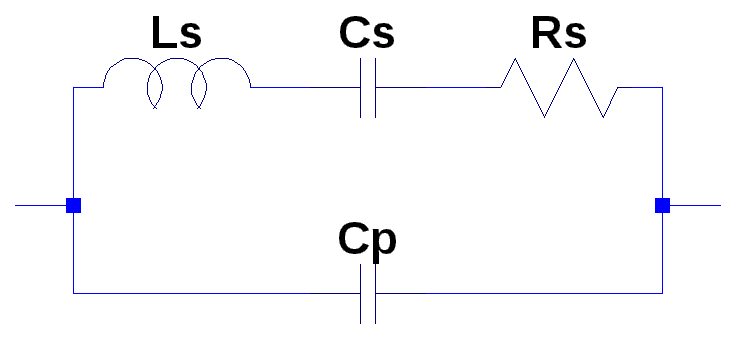
\includegraphics[width=8cm]{Imagenes/esqXtal.png}
			\caption{Esqemático simplificado del cristal.}
			\label{img004} 
		\end{figure}

		\indent Dicho circuito equivalente posee dos frecuencias de resonancia,
		una serie y otra paralelo, ambas muy cercanas entre sí. La resonancia 
		serie es la menor de las dos, en dicho punto la fase de la impeancia es
		igual a 0, por ende, puede medirse directamente la resistencia serie 
		$R_s$. \\
		\indent Como generalmente la resistencia de la resonancia serie es muy 
		chica, hay que restar $0.5\Omega$ del efecto de carga de la punta. \\
		\indent Un gráfico típico de la impeancia de entrada de un xtal en 
		función de la frecuencia se observa en la imagen \ref{img005}.
		%ffRANnnnnnnnnnnnn sacale el fondo gris!!!!!!!!!!!!!!!!!!!!!!!!
		\begin{figure}[!htb]
			\centering
			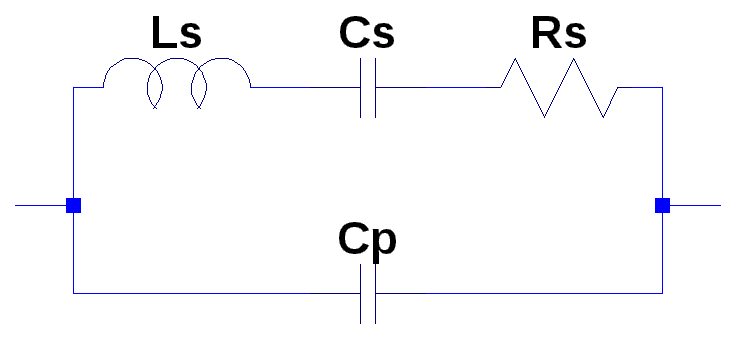
\includegraphics[width=8cm]{Imagenes/esqXtal.png}
			\caption{Impedancia típica de un xtal en función de la frecuencia.}
			\label{img005} 
		\end{figure}

		\indent Se puede observar que el circuito se comporta como un capacitor
		a frecuencias menores uqe la de la resonancia serie, dicho capacitor es 
		aproximadamente igual a $C_p$ dado que $C_s$ es mucho menor. \\
		\indent Las otras fórmulas utilizadas para realizar los cálculos del 
		resto de los parámetros del xtal son las siguientes.
		
		$$C_p = \frac{1}{2\omega\cdot x_c}$$
		$$C_s = C_p \frac{2\cdot(f_p - f_s)}{f_p}$$
		$$L = \frac{1}{4\pi^2f_s^2C_s}$$

		\indent Donde $f_s$ y $f_p$ son las frecuencias de resonancia serie y 
		paralelo respctivamente. \\
		\indent A la hora de medir el Q del cristal se determina utilizando el 
		método del ancho de banda, el cual consiste en medir las frecuencias 
		donde la pontencia de salida disminuye unos $3db$, o que es lo mismo, 
		si se trata de un polo simple como este caso, hay un defasaje de $45º$.
		Por lo tanto Q queda determinado de la siguiente forma
		$$Q = \frac{f_0}{\Delta f_{\pm45}}$$
		\indent Para realizar la medición de los parámetros se utiliza el 
		impedancímetro vectorial (hp 5100A), el cual mide la fase y el módulo de
		la impedancia. Los valores obtenidos se vuelcan en la tabla \ref{tab003}

		\begin{table}[!htp]
			\centering
			\begin{tabular}{|c|c|c|}
				\hline
				Frecuencia [MHz] & |Z| & arg(Z) \\
				\hline
				18.9960000 & $2.85~K\Omega$ & $-90^{\circ}$ \\
				\hline
				19.9948400 & - & $-45^{\circ}$ \\ 
				\hline
				19.9950580 & $17~\Omega$ & $0^{\circ}$ \\
				\hline
				19.9952860 & - & $45^{\circ}$ \\ 
				\hline									
				20.0311383 & $560~\Omega$ & $45^{\circ}$ \\
				\hline									
				20.0311556 & $640~\Omega$ & $0^{\circ}$ \\
				\hline									
				20.0311634 & $550~\Omega$ & $-45^{\circ}$ \\
				\hline									
			\end{tabular}
			\caption{Mediciones con el impedancímetro vectorial} \label{tab003}
		\end{table}	

		\subsubsection{Mediciones en un circuito activo}
			
	\section{Conclusiones}
	\indent Viva Venezuela!\\
\end{document}

